\newcommand{\pd}[2]{\displaystyle\frac{\displaystyle\partial #1}{\displaystyle\partial #2}}
\newcommand{\vol}[1]{\langle #1 \rangle}
\newcommand{\sigy}{\sigma_{\rm y}}
\newcommand{\epse}{\varepsilon^{\rm e}}
\newcommand{\epsp}{\varepsilon^{\rm p}}

\newcommand{\epst}{\varepsilon}
\newcommand{\sig}{\sigma}
\newcommand{\Fp}{f^{\rm p}}
\newcommand{\Fd}{f^{\rm d}}
\newcommand{\norm}[1]{| #1 |}

\section{Motivation}

\frame{\frametitle{Fatigue damage}

\uncover<1->{
		\twocol{	\begin{itemize}
				\item Cyclic loading
			\end{itemize}
			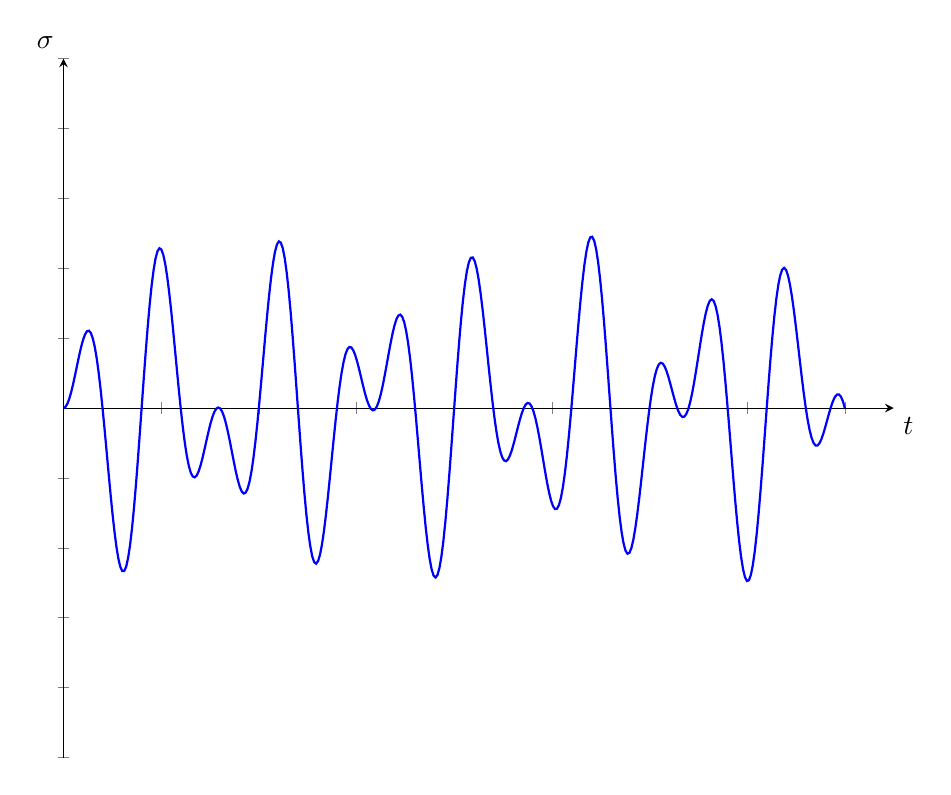
\begin{tikzpicture}[scale=1]
			\begin{axis}[axis x line=center, axis y line=center,
			xticklabels={},yticklabels={},xlabel style={below right},
			ylabel style={above left},ymin=-1,ymax=1,xmin=0,xmax=8.5,
			width=\textwidth,xlabel=$t$,ylabel=$\sigma$]
			\addplot [color=blue,thick,mark=none,domain=0:8,samples=400]{sin(2*\x r)*0.5*sin(pi / 2 * 5 * \x r)} ;
			\end{axis}
			\end{tikzpicture}
		}{
			\centering
			\uncover<2->{\hfil
				\begin{itemize}
					\item Damage
				\end{itemize}
				
					\only<2>{\includegraphics[width=0.9\textwidth]{./img/Windturbine.jpg}\\[-0.3cm]}

					\only<3->{\includegraphics[width=0.9\textwidth]{./img/bridge.jpg}\\[-0.3cm]}
					\uncover<2-3>{\vspace*{0.1cm} {\tiny Image by alegri / 4freephotos.com}}
		
				}
				
				}
			}
			{
			
			}
	}



\frame{\frametitle{Fatigue damage}
	
		\twocol{	\begin{itemize}
				\item Cyclic loading
			\end{itemize}
			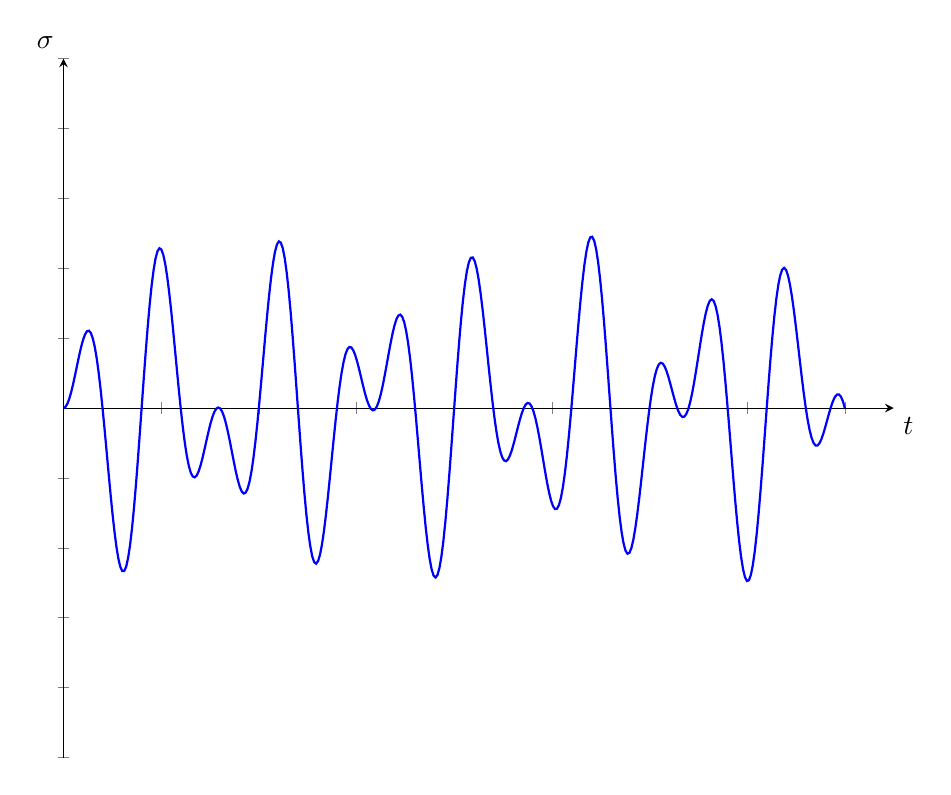
\begin{tikzpicture}[scale=1]
			\begin{axis}[axis x line=center, axis y line=center,
			xticklabels={},yticklabels={},xlabel style={below right},
			ylabel style={above left},ymin=-1,ymax=1,xmin=0,xmax=8.5,
			width=\textwidth,xlabel=$t$,ylabel=$\sigma$]
			\addplot [color=blue,thick,mark=none,domain=0:8,samples=400]{sin(2*\x r)*0.5*sin(pi / 2 * 5 * \x r)} ;
			\end{axis}
			\end{tikzpicture}
		}{
			\centering
			\uncover<1->{\hfil
				\uncover<1->{	\begin{itemize}
						{\item Virtual experiments\\[0.5cm]}
						{\item Continuum damage model\\[0.5cm]}
						{\item Millions of cycles\\[0.5cm]}
						{\item Computationally expensive\\[0.5cm]}
					\end{itemize}}	
				}
			}
			{
				\uncover<2>{
					\begin{block}{ \centering Model order reduction (MOR) techniques}
					\end{block}
					
				}
			}
		}

	
\section{LATIN framework}

\frame{\frametitle{LATIN overview}
	\begin{center}
		\includegraphics[width=0.6\textwidth,clip]{./fig/latin_iter.pdf}\\	
		{Illustration of the LATIN iterations}
	\end{center}
}

\frame{\frametitle{LATIN with two-time scale for ductile damage}
		\begin{itemize}
			\item The first and second nodal cycles are computed
			\begin{center}
				\includegraphics[width=0.6\textwidth]{./fig/2scale.png}
			\end{center}
			\item The initial condition QoI are interpolated between the
			nodal cycles
	\end{itemize}
		
%		\mediabutton[jsaction={anim.myAnim.playFwd();}]{\fbox{\strut Play}}
%		\mediabutton[jsaction={anim.myAnim.pause();}]{\fbox{\strut Pause}}
	%		 \includegraphics[width=0.4\linewidth]{./img/lating-0.png}
\begin{center}
	\includegraphics[width=0.7\textwidth]{./fig_new/inter.png}\\[-0.3cm]	
\end{center}

}

\frame{\frametitle{Ductile damage example}
%	\begin{itemize}
%		\item The first nodal cycle is simulated
%		\item The initial condition for the next
%		cycle is based on the damage
%		evolution equation
%		\item QoI are interpolated between the
%		nodal cycles
%	\end{itemize}
	
	%		\mediabutton[jsaction={anim.myAnim.playFwd();}]{\fbox{\strut Play}}
	%		\mediabutton[jsaction={anim.myAnim.pause();}]{\fbox{\strut Pause}}
	%		 \includegraphics[width=0.4\linewidth]{./img/lating-0.png}
		\begin{center}
		\begin{tikzpicture}[x=1cm,y=1cm,scale=0.7]
	
	%{ \small
	%	\node at (4,-2) [align=left]	{
	%	\only<1>{$\ \psi = \frac{1}{2} \ E \ (\epse)^2 + \underset{\text{hardening}}{\underbrace{ \frac{1}{2} \ C \ (\alpha)^2}} $\\[0.2cm]}
	%	\only<2->{$\psi = \frac{1}{2} \ E \ (\epse)^2 \ {\color{red} (1-D)} + \underset{\text{hardening}}{\underbrace{ \frac{1}{2} \ C \ (\alpha)^2}}$\\[0.2cm] \hspace*{0.0cm}}
	%	$\phi=\phi^{\rm p} \uncover<3->{+ \color{red}  \phi^{\rm d}}$\\[0.2cm]
	%	\begin{tabular}{ll}
	%	$ \phi^{\rm p}= \frac{k}{n+1} \vol{f^{\rm p}}_+^{n+1}$ & $f^{\rm p} = \norm{\sigma - \beta} + \frac{a}{C} \ \beta^2 - \sigy$ \\[0.2cm]
	%	\uncover<4->{$ \phi^{\rm d} = \frac{\kd}{\nd+1} \vol{\Fd}_+^{\nd+1}$ &  $ \Fd=Y-Y_0$}
	%	\end{tabular}
	%
	%	};
	%}
	\fill [ultra thick] (0,-0.05+1.75) rectangle (4,0.05+1.75) node [above,pos=0.5] {};
	\fill [ultra thick] (0,-0.05+1.25) rectangle (4,0.05+1.25) node [above,pos=0.5] {};
	\fill [thick] (4,-0.05+1.25) rectangle (4.05,0.05+1.75) node [above,pos=0.5] {};
	
	\draw [->,thin] (4,0+1.5) -- (4.5,0+1.5) node [below right,pos=0.5] {$\bar{u}$};
	\draw [ultra thick] (0,-0.5+1.5) -- (0,0.5+1.5);
	\path [pattern=north west lines] (-0.25,-0.5+1.5) rectangle (0,0.5+1.5);
	\begin{axis}[at={(0.6\textwidth,-2)},axis x line=center, axis y line=center,
	xticklabels={},yticklabels={},xlabel style={below right},
	ylabel style={above left},ymin=-1,ymax=1,xmin=0,xmax=8.5,
	width=0.5\textwidth,xlabel=$t$,ylabel=$\bar{u}$]
	\addplot [color=blue,thick,mark=none,domain=0:8,samples=400]{0.5*sin(pi / 2 * 5 * \x r)} ;
	\end{axis}
	\end{tikzpicture}\\

		\includegraphics[width=0.5\textwidth]{./fig/2scale_damage.png}
		\hfill
		\includegraphics[width=0.45\textwidth]{./fig/2scale_speed.png}
	\end{center}
	
}

\frame{\frametitle{LATIN for brittle damage}
		\begin{flushleft}
			\only<1>{
				\begin{itemize}
					\item {Assumptions}\\[0.2cm]
					\begin{itemize}
						\item Free energy function $\psi_{\rm e}  = 1/2 \ (1-D) \ E \ (\epse)^2$
						\item Damage dissipation potential
						\begin{equation*}
						\varphi_{\rm d} = \frac{\kd}{\nd+1} \vol{\Fd}_+^{\nd+1}, \qquad \Fd=Y-Y_0
%%							\phid = \frac{\kd}{\nd+1} \vol{\Fd}_+^{\nd+1}, \qquad \Fd=Y-Y_0, 
%							%	\qquad Y_0 = \frac{\sigma_{\rm y}^2}{2 \ E}
						\end{equation*}
						 $Y_0$ is the initial damage limit and $\kd$ and $\nd$ are the damage viscous parameters. 
					\end{itemize}
				\end{itemize}
			}	
		\end{flushleft}
}


\frame{\frametitle{LATIN scheme for brittle damage}
	\begin{flushleft}
		\begin{itemize}
			\item The strain and displacement are initialised by the given B.C. only
			\item Global stage\\
			Purely elastic and the displacement is written in PGD form
			\begin{itemize}
				\item The static admissibility
					\begin{equation*}
					\int \sigma \ \varepsilon^\ast \ \d \Omega \d t = \int b \ u^\ast \ \d \Omega \d t + \int_{\partial\Omega_N} \bar{t} \ u^\ast \ \d s \d t.
					\end{equation*}
					\item In terms of corrections it becomes
					\begin{equation*}
					\int \Delta \sigma \ \varepsilon^\ast \ \d \Omega \d t = 0. 
					\label{bd:sa0}
					\end{equation*}
			\end{itemize}
		\end{itemize}	
	\end{flushleft}
}

\frame{\frametitle{LATIN scheme for brittle damage}
	\begin{flushleft}
		\begin{itemize}
			\item Global search direction
			\begin{align*}
			&( \stepk[e]{\varepsilon} -  \stepj[e]{\varepsilon} )- E^{-1} (\stepk[]{\sigma} -\stepj[]{\sigma}) = 0,\\
			&\Delta \stepk[e]{\varepsilon} - E^{-1} \Delta\stepk[]{\sigma} - \hf^{\rm e}=0,\\
			&\hf^{\rm e} = - E^{-1} (\stepj{\sigma}-\stepi{\sigma}) + (\stepj[e]{\varepsilon}-\stepi[e]{\varepsilon}).
			\end{align*}
			\item Separate representation of the displacement
			\begin{equation*}
			\Delta u = \lambda \ v, \qquad \Delta \varepsilon = \lambda \ \bar{\varepsilon} = \lambda \ \grad{v},
			\end{equation*}
			leads to the following variations
			\begin{equation*}
			\Delta u^\ast = \lambda^\ast \ v + \lambda \ v^\ast, \qquad \Delta \varepsilon^\ast = \lambda^\ast \ \grad{v} + \lambda \ \grad{v}^\ast.
			\end{equation*}
		\end{itemize}	
	\end{flushleft}
}

\frame{\frametitle{LATIN scheme for brittle damage}
	\begin{flushleft}
		\begin{itemize}
			\item Static admissibility as a space and a time problems 
			\begin{align*}
			& \int \grad{v}^\ast \left( \int \lambda \ \rC \ \lambda \d t \right) \grad{v} \d \Omega = \int  \left( \int \hf^{\rm e} \ \rC \ \lambda \d t \right) \grad{v}^\ast \d \Omega,\\
			& \int \lambda^\ast \left( \int  \grad{v} \ \rC \ \grad{v} \d \Omega \right) \lambda  \d t = \int \lambda^\ast \left( \int \hf^{\rm e} \ \rC \ \grad{v} \d \Omega \right)  \d t.
			\end{align*} 
			\item The strain space function can be computed through the kinematic admissibility relation as $\bar{\varepsilon} = \grad{v}$.\\
	
		\item Local stage
		\begin{itemize}
			\item The stress is taken from the last global stage
			\item The damage evolution is computed
		\end{itemize}
		\vfill
	\end{itemize}
	\begin{equation*}
	\begin{split}
	{\dot{D}} &= \pd{\varphi_{\rm d}}{Y}= \kd  \vol{\Fd}_+^{\nd}
	\end{split}
	\end{equation*} 	
	\end{flushleft}
}

\frame{\frametitle{Brittle damage example}
	\begin{itemize}
		\item Constant amplitude loading and adaptive time jumps
	\end{itemize}	
	\begin{center}
		\includegraphics[width=0.8\textwidth]{./fig_new/img-100.png}
	\end{center}
}

\frame{\frametitle{Brittle damage example}
	\begin{itemize}
		\item Constant amplitude loading and adaptive time jumps
	\end{itemize}	
	\begin{center}
		\includegraphics[width=0.5\textwidth]{./fig/brittle_damage.png}
		\hfill
		\includegraphics[width=0.5\textwidth]{./fig/brittle_damage_evolution.png}
	\end{center}
}

\frame{\frametitle{Variable loading}
	\begin{itemize}
		\item L-H and H-L sequence
		
		\begin{center}
			\includegraphics[width=0.45\textwidth]{./fig_new/blockloading.eps}
			\hfil
			\includegraphics[width=0.55\textwidth]{./fig_new/LH_HL_brittle_damage.png}
		\end{center}
		
		\item Time modes are scaled to have a better initialisation
	\end{itemize}
}

\frame{\frametitle{Modes optimisation}
		\begin{itemize}
		\item Modified Gram Schmidt and SVD
		\end{itemize}	
	\begin{center}
		\includegraphics[width=0.5\textwidth]{./fig/modified_gram_schmidt_space.png}
		\hfill
		\includegraphics[width=0.5\textwidth]{./fig/svd_space.png}
	\end{center}
}

\frame{\frametitle{Modes truncation}
	\begin{center}
		\includegraphics[width=0.5\textwidth]{./fig/singular_values_decay.png}
		\hfill
		\includegraphics[width=0.5\textwidth]{./fig/svd_space_compressed.png}
	\end{center}
}

\frame{ \frametitle{Conclusion and current research}
	\begin{itemize}
		\item MOR approach for HCF
		\item It works for variable loading
	\end{itemize}
	\begin{block}{\centering Current objectives}\end{block}
	\begin{itemize}
		\item Virtual S-N curves
		\item Modes selection and optimisation for variable loading
		\item Reference point method or hyper-reduction
		\item Parametric loading
		\item Time homogenisation
	\end{itemize}
}


\newcommand{\chronoperiode}[5]{
	\pgfmathsetmacro{\first}{#2 - .98} % beginig of the peropd
	\pgfmathsetmacro{\last}{(#3 - 1.02} % end of the period
	\pgfmathsetmacro{\middle}{(\first+\last)/2} % position of the country name
	\fill[#5] (\first,#4-1+0.05) rectangle (\last,#4-0.05) (\middle,#4-.5) node[white, font=\sf]{#1};
}
\frame{\frametitle{Milestone plan}
	
	\begin{center}
		\begin{itemize}
			\item {First year}\\
			{\color{gray} Constitutive modelling, LATIN-PGD and Two-time scale}
			\item { Second year}\\
			{\color{gray} Brittle damage and different amplitudes} and {\color{luhBlue} RPM}
			\item {Third year}\\
			 {\color{luhBlue} Parametric PGD and Computations and thesis writing}
		\end{itemize}
	\end{center}
	\uncover<2>{\begin{block}{\centering Thank you for your attention!}
	\end{block}}
}

\frame{
	\begin{itemize}
		\item Time comparison\\
			{ \scriptsize D. N\'{e}ron et al, Time-space PGD for the rapid solution of 3D nonlinear
			parametrized problems in the many-query context, \textit{IJNME}, 2015.}
	\end{itemize}
	}
	

\frame{
	\begin{itemize}
		\item LATIN convergence conditions\\
		{\scriptsize Ladeveze 1999 [p84]}\\
	\end{itemize}
}

\frame{
	\begin{itemize}
		\item PGD existence and convergence\\
		{\scriptsize Ladeveze 1999 [p119]}\\[0.5cm]
		\item  PGD for solving PDE\\
		{\scriptsize A. Nouy. A priori model reduction through proper generalized decomposition for solving time-dependent partial differential equations. Computer Methods In Applied Mechanics and Engineering, 199(23- 24):1603–1626, 2010.}\\[0.5cm]
		{\scriptsize Antonio Falco}\\
	\end{itemize}
}

\frame{\frametitle{Different loading sequence}
	\begin{center}
	\includegraphics[width=0.8\textwidth]{./fig/damage_evolution}
	\end{center}
}
\frame{\frametitle{Different loading sequence with elastic loading}
	\begin{center}
		\includegraphics[width=0.8\textwidth]{./fig/damage_evolution2}
	\end{center}
}
\frame{\frametitle{The used mesh}
	\begin{center}
		\includegraphics[width=0.8\textwidth]{./fig/mesh.png}
	\end{center}
}
	
%\frame{\frametitle{}
%	
%	}
	
\input{MOR}
%\frame{
%	\begin{itemize}
%		
%		\item PGD convergence\\
%		generalisation of the POD of a given function, is independent of the LATIN-PGD. In the book, you have this proof for a given continuous function, 
%		[Ladevèze 99] 
%		
%	\end{itemize}
%}

%\frame[plain]{
%	
%	\frametitle{Milestone plan}
%	
%	\begin{center}
%		\only<1->{
%			\scalebox{0.48}[0.6]{
%				\hspace*{-1cm}
%				\begin{tikzpicture}[x=20mm,y=7mm]
%				\draw[help lines] (0,0) grid[step=1] (12,2);
%				\renewcommand\a{1}
%				\renewcommand\aa{2016}
%				\draw[gray] (3*\a-3,0) -- +(0,-7mm) node[pos=.5, below right, inner sep=1pt]{$\aa$};
%				\foreach[count=\m] \mm in {O,N,D}
%				\node[font=\tiny,below,gray] at (12*\a+\m-12.5,0) {\mm};
%				\renewcommand\a{2}
%				\renewcommand\aa{2017}
%				\draw[gray] (3*\a-3,0) -- +(0,-7mm) node[pos=.5, below right, inner sep=1pt]{$\aa$};
%				\foreach[count=\m] \mm in {J,F,M,A,M,J,J,A,S}
%				\node[font=\tiny,below,gray] at (3*\a+\m-3.5,0) {\mm};	
%				
%				plot the data
%				\chronoperiode{LATIN}{1}{2}{1}{gray}
%				\chronoperiode{MATLAB}{1}{2}{2}{gray}
%				\chronoperiode{Constitutive modelling}{2}{4}{1}{gray}
%				\chronoperiode{LATIN + PGD}{4}{6}{1}{gray}
%				\chronoperiode{MATLAB}{4}{6}{2}{gray}
%				\chronoperiode{MOR in time}{6}{8}{1}{luhBlue}
%				\chronoperiode{Different amplitudes}{8}{13}{1}{luhBlue}
%				
%				\chronoperiode{LMT}{7}{10}{2}{lightgray}
%				\chronoperiode{LMT}{12}{13}{2}{lightgray}
%				\end{tikzpicture}
%			}
%			\vfill
%			\scalebox{0.48}[0.6]{
%				\hspace*{-1cm}
%				\begin{tikzpicture}[x=20mm,y=7mm]
%				
%				\draw[help lines] (0,0) grid[step=1] (12,2);
%				\renewcommand\a{1}
%				\renewcommand\aa{2017}
%				\draw[gray] (3*\a-3,0) -- +(0,-7mm) node[pos=.5, below right, inner sep=1pt]{$\aa$};
%				\foreach[count=\m] \mm in {O,N,D}
%				\node[font=\tiny,below,gray] at (12*\a+\m-12.5,0) {\mm};
%				\renewcommand\a{2}
%				\renewcommand\aa{2018}
%				\draw[gray] (3*\a-3,0) -- +(0,-7mm) node[pos=.5, below right, inner sep=1pt]{$\aa$};
%				\foreach[count=\m] \mm in {J,F,M,A,M,J,J,A,S}
%				\node[font=\tiny,below,gray] at (3*\a+\m-3.5,0) {\mm};	
%				
%				plot the data
%				\chronoperiode{Different frequencies}{1}{7}{1}{luhBlue}
%				\chronoperiode{Random loading}{7}{13}{1}{luhBlue}
%				
%				\chronoperiode{LMT}{1}{2}{2}{lightgray}
%				\chronoperiode{LMT}{7}{10}{2}{lightgray}
%				
%				
%				\end{tikzpicture}	
%			}
%			
%			\vfill
%			\scalebox{0.48}[0.6]{
%				\hspace*{-1cm}
%				\begin{tikzpicture}[x=20mm,y=7mm]
%				
%				\draw[help lines] (0,0) grid[step=1] (12,2);
%				\renewcommand\a{1}
%				\renewcommand\aa{2018}
%				\draw[gray] (3*\a-3,0) -- +(0,-7mm) node[pos=.5, below right, inner sep=1pt]{$\aa$};
%				\foreach[count=\m] \mm in {O,N,D}
%				\node[font=\tiny,below,gray] at (12*\a+\m-12.5,0) {\mm};
%				\renewcommand\a{2}
%				\renewcommand\aa{2019}
%				\draw[gray] (3*\a-3,0) -- +(0,-7mm) node[pos=.5, below right, inner sep=1pt]{$\aa$};
%				\foreach[count=\m] \mm in {J,F,M,A,M,J,J,A,S}
%				\node[font=\tiny,below,gray] at (3*\a+\m-3.5,0) {\mm};	
%				
%				plot the data
%				\chronoperiode{Computations and parametric study}{1}{7}{1}{luhBlue}
%				\chronoperiode{Thesis writing}{7}{13}{1}{luhBlue}
%				
%				\chronoperiode{LMT}{1}{2}{2}{lightgray}
%				\chronoperiode{LMT}{7}{10}{2}{lightgray}
%				\end{tikzpicture}	
%			}
%		}	
%		\uncover<2>{	\begin{block}{\centering Thank you for your attention!}
%		\end{block}}
%	\end{center}
%}